% Options for packages loaded elsewhere
\PassOptionsToPackage{unicode}{hyperref}
\PassOptionsToPackage{hyphens}{url}
\PassOptionsToPackage{dvipsnames,svgnames,x11names}{xcolor}
\documentclass[
  11pt,
  a4paper,
]{article}
\usepackage{xcolor}
\usepackage[margin=2.5cm]{geometry}
\usepackage{amsmath,amssymb}
\setcounter{secnumdepth}{-\maxdimen} % remove section numbering
\usepackage{iftex}
\ifPDFTeX
  \usepackage[T1]{fontenc}
  \usepackage[utf8]{inputenc}
  \usepackage{textcomp} % provide euro and other symbols
\else % if luatex or xetex
  \usepackage{unicode-math} % this also loads fontspec
  \defaultfontfeatures{Scale=MatchLowercase}
  \defaultfontfeatures[\rmfamily]{Ligatures=TeX,Scale=1}
\fi
\usepackage{lmodern}
\ifPDFTeX\else
  % xetex/luatex font selection
\fi
% Use upquote if available, for straight quotes in verbatim environments
\IfFileExists{upquote.sty}{\usepackage{upquote}}{}
\IfFileExists{microtype.sty}{% use microtype if available
  \usepackage[]{microtype}
  \UseMicrotypeSet[protrusion]{basicmath} % disable protrusion for tt fonts
}{}
\makeatletter
\@ifundefined{KOMAClassName}{% if non-KOMA class
  \IfFileExists{parskip.sty}{%
    \usepackage{parskip}
  }{% else
    \setlength{\parindent}{0pt}
    \setlength{\parskip}{6pt plus 2pt minus 1pt}}
}{% if KOMA class
  \KOMAoptions{parskip=half}}
\makeatother
\usepackage{longtable,booktabs,array}
\newcounter{none} % for unnumbered tables
\usepackage{calc} % for calculating minipage widths
% Correct order of tables after \paragraph or \subparagraph
\usepackage{etoolbox}
\makeatletter
\patchcmd\longtable{\par}{\if@noskipsec\mbox{}\fi\par}{}{}
\makeatother
% Allow footnotes in longtable head/foot
\IfFileExists{footnotehyper.sty}{\usepackage{footnotehyper}}{\usepackage{footnote}}
\makesavenoteenv{longtable}
\usepackage{graphicx}
\makeatletter
\newsavebox\pandoc@box
\newcommand*\pandocbounded[1]{% scales image to fit in text height/width
  \sbox\pandoc@box{#1}%
  \Gscale@div\@tempa{\textheight}{\dimexpr\ht\pandoc@box+\dp\pandoc@box\relax}%
  \Gscale@div\@tempb{\linewidth}{\wd\pandoc@box}%
  \ifdim\@tempb\p@<\@tempa\p@\let\@tempa\@tempb\fi% select the smaller of both
  \ifdim\@tempa\p@<\p@\scalebox{\@tempa}{\usebox\pandoc@box}%
  \else\usebox{\pandoc@box}%
  \fi%
}
% Set default figure placement to htbp
\def\fps@figure{htbp}
\makeatother
\setlength{\emergencystretch}{3em} % prevent overfull lines
\providecommand{\tightlist}{%
  \setlength{\itemsep}{0pt}\setlength{\parskip}{0pt}}
\usepackage{bookmark}
\IfFileExists{xurl.sty}{\usepackage{xurl}}{} % add URL line breaks if available
\urlstyle{same}
\hypersetup{
  colorlinks=true,
  linkcolor={blue},
  filecolor={Maroon},
  citecolor={Blue},
  urlcolor={blue},
  pdfcreator={LaTeX via pandoc}}

\author{}
\date{}

\begin{document}

% --- Title page (group + title only) ---
\begin{titlepage}
\centering
\vspace*{1cm}
\IfFileExists{uiimages/Logo-Complet-ESI-SBA-200mm-x-200mm_couleur-1024x1024.png}{%
  \pandocbounded{
\includegraphics[width=0.42\textwidth,keepaspectratio]{uiimages/Logo-Complet-ESI-SBA-200mm-x-200mm_couleur-1024x1024.png}}\\[1.5cm]%
}{%
  \textit{\small (Add \texttt{uiimages/Logo-Complet-ESI-SBA-200mm-x-200mm\_couleur-1024x1024.png} next to \texttt{REPORT.tex} to show the school logo.)}\\[1.5cm]%
}
{\LARGE\bfseries Computer Vision Cube Solver\par}
\vspace{0.75cm}
{\large Project Report\par}
\vspace{4cm}
{\large\bfseries Group members\par}
\vspace{1.5cm}
\begin{minipage}{0.65\textwidth}
\centering
\begin{tabular}{@{}ll@{}}
\textbf{DIB} & Mehdi \\
\textbf{BENDAIA} & Abderrahmane \\
\end{tabular}
\end{minipage}
\vspace{1.8cm}
{\small\textbf{Source code repository}\par}
\vspace{0.35em}
{\small\url{https://github.com/laponjade/computer_vision_cube_solver}\par}
\vfill
\end{titlepage}

\clearpage
% --- Table of contents on its own page(s) ---
{
\setcounter{tocdepth}{3}
\tableofcontents
}
\clearpage
% --- Main report body begins here (separate from title / TOC) ---
\section{1. Introduction}\label{introduction}

This report documents the iterative engineering process behind a
computer vision pipeline that captures a Rubik's cube from a live camera
feed and reconstructs its full 54-sticker state for downstream solving.
The work focuses on two complementary problems:

\begin{enumerate}
\def\labelenumi{\arabic{enumi}.}
\tightlist
\item
  \textbf{Detecting the cube face} in arbitrary photos and isolating its
  3x3 grid in a normalized perspective.
\item
  \textbf{Classifying the color} of each of the 9 stickers per face
  robustly, under varying lighting, exposure, white balance, and camera
  quality.
\end{enumerate}

Multiple modeling approaches were attempted before converging to a final
pipeline that achieves high accuracy and is robust to real-world
conditions. Each stage below describes the motivation, the methodology,
the failure modes that emerged, and the quantitative or qualitative
evidence that informed the next iteration.

\begin{center}\rule{0.5\linewidth}{0.5pt}\end{center}

\section{2. System Overview}\label{system-overview}

The final pipeline follows a two-stage design:

\begin{verbatim}
camera frame
    -> [Stage 1] Cube face detector (YOLO-OBB)
    -> oriented bounding quad of the face
    -> perspective warp + 3x3 grid sampling
    -> 9 sticker crops per face
    -> [Stage 2] Sticker color classifier
    -> face state (3x3 of canonical colors)
\end{verbatim}

Stage 1 produces a tight, oriented region of interest. Stage 2 ingests
the 9 normalized sticker crops and returns one of six canonical colors
per sticker. The final 3x3 face is then composed with the rest of the
cube and passed to a solver.

\begin{center}\rule{0.5\linewidth}{0.5pt}\end{center}

\section{3. Stage 1 --- Cube Face Detection (Oriented Object
Detection)}\label{stage-1-cube-face-detection-oriented-object-detection}

\subsubsection{3.1 Motivation}\label{motivation}

Detecting only the \textbf{front face} of the cube --- rather than the
full cuboid silhouette --- gives the next stage a clean, planar surface
to sample stickers from. To support natural hand-held framing where the
cube is rarely perfectly axis-aligned, an \textbf{oriented bounding box}
model was chosen over a standard axis-aligned detector. The oriented
quadrilateral allows a downstream perspective warp into a square canvas,
after which the 3x3 grid is trivially extracted.

\subsubsection{3.2 Approach}\label{approach}

A pretrained YOLO oriented-object-detection (OBB) backbone was
fine-tuned on a curated dataset of cube photos. Each image was annotated
with a quadrilateral around the visible face. Standard data augmentation
was enabled (horizontal flip, scale jitter, color jitter, mosaic, random
erasing) and training was carried out on a single accelerator device for
50 epochs at 640 x 640 resolution.

\subsubsection{3.3 Qualitative Results}\label{qualitative-results}

The training and validation batches show the model learning to localize
the face under varied perspectives, partial occlusions, and lighting.

{\def\LTcaptype{none} % do not increment counter
\begin{longtable}[]{@{}
  >{\raggedright\arraybackslash}p{(\linewidth - 2\tabcolsep) * \real{0.5000}}
  >{\raggedright\arraybackslash}p{(\linewidth - 2\tabcolsep) * \real{0.5000}}@{}}
\toprule\noalign{}
\begin{minipage}[b]{\linewidth}\raggedright
Stage
\end{minipage} & \begin{minipage}[b]{\linewidth}\raggedright
Visualization
\end{minipage} \\
\midrule\noalign{}
\endhead
\bottomrule\noalign{}
\endlastfoot
Training batch (early) &
\pandocbounded{\includegraphics[keepaspectratio,alt={Train batch 0}]{runs/obb/rubik_cube_from_best/train_batch0.jpg}} \\
Training batch (late) &
\pandocbounded{\includegraphics[keepaspectratio,alt={Train batch late}]{runs/obb/rubik_cube_from_best/train_batch400.jpg}} \\
Validation labels &
\pandocbounded{\includegraphics[keepaspectratio,alt={Validation labels}]{runs/obb/rubik_cube_from_best/val_batch0_labels.jpg}} \\
Validation predictions &
\pandocbounded{\includegraphics[keepaspectratio,alt={Validation predictions}]{runs/obb/rubik_cube_from_best/val_batch0_pred.jpg}} \\
Per-class label distribution &
\pandocbounded{\includegraphics[keepaspectratio,alt={Label distribution}]{runs/obb/rubik_cube_from_best/labels.jpg}} \\
\end{longtable}
}

\subsubsection{3.4 Quantitative Results}\label{quantitative-results}

The model converges quickly and reaches high precision and recall. The
training curves and operating-point analyses are summarized below.

{\def\LTcaptype{none} % do not increment counter
\begin{longtable}[]{@{}
  >{\raggedright\arraybackslash}p{(\linewidth - 2\tabcolsep) * \real{0.5000}}
  >{\raggedright\arraybackslash}p{(\linewidth - 2\tabcolsep) * \real{0.5000}}@{}}
\toprule\noalign{}
\begin{minipage}[b]{\linewidth}\raggedright
Metric
\end{minipage} & \begin{minipage}[b]{\linewidth}\raggedright
Plot
\end{minipage} \\
\midrule\noalign{}
\endhead
\bottomrule\noalign{}
\endlastfoot
Overall training/validation curves &
\pandocbounded{\includegraphics[keepaspectratio,alt={Training curves}]{runs/obb/rubik_cube_from_best/results.png}} \\
Precision--Recall curve (oriented box) &
\pandocbounded{\includegraphics[keepaspectratio,alt={PR curve}]{runs/obb/rubik_cube_from_best/BoxPR_curve.png}} \\
F1 vs.~confidence &
\pandocbounded{\includegraphics[keepaspectratio,alt={F1 curve}]{runs/obb/rubik_cube_from_best/BoxF1_curve.png}} \\
Precision vs.~confidence &
\pandocbounded{\includegraphics[keepaspectratio,alt={P curve}]{runs/obb/rubik_cube_from_best/BoxP_curve.png}} \\
Recall vs.~confidence &
\pandocbounded{\includegraphics[keepaspectratio,alt={R curve}]{runs/obb/rubik_cube_from_best/BoxR_curve.png}} \\
Confusion matrix &
\pandocbounded{\includegraphics[keepaspectratio,alt={Confusion matrix}]{runs/obb/rubik_cube_from_best/confusion_matrix.png}} \\
Confusion matrix (normalized) &
\pandocbounded{\includegraphics[keepaspectratio,alt={Confusion matrix normalized}]{runs/obb/rubik_cube_from_best/confusion_matrix_normalized.png}} \\
\end{longtable}
}

\textbf{Headline numbers (final epoch):}

\begin{itemize}
\tightlist
\item
  Precision \textasciitilde{} 0.97
\item
  Recall \textasciitilde{} 0.94
\item
  mAP@0.5 \textasciitilde{} 0.98
\item
  mAP@0.5:0.95 \textasciitilde{} 0.96
\end{itemize}

The detector is therefore a reliable upstream component: it produces a
clean oriented quadrilateral that can be warped into a normalized face
crop for the color stage.

\begin{center}\rule{0.5\linewidth}{0.5pt}\end{center}

\section{4. Stage 2 --- Sticker Color Recognition
(Iterations)}\label{stage-2-sticker-color-recognition-iterations}

The color stage proved to be substantially harder than the detection
stage. Three distinct approaches were attempted before the pipeline
reached production-quality robustness.

\subsubsection{4.1 First attempt --- Whole-face image
classifier}\label{first-attempt-whole-face-image-classifier}

\paragraph{Approach}\label{approach-1}

A classification model was trained on whole sticker / face photographs
collected in unconstrained conditions. The model was fed
\emph{uncropped} sticker regions and asked to output the dominant color
directly. The training set contained images of plain colored objects in
addition to stickers, with substantial variability in framing, exposure,
and backgrounds.

\paragraph{Why it underperformed}\label{why-it-underperformed}

Without a precise, repeatable crop around each sticker:

\begin{itemize}
\tightlist
\item
  The model often latched onto background pixels (skin, table, holder).
\item
  Mixed exposures across frames pushed similar sticker colors (e.g.~red
  / orange, green / blue under cool white balance) into overlapping
  regions of feature space.
\item
  The model had no explicit signal about \emph{where} in the image the
  sticker was; it had to learn detection and classification
  simultaneously, which is data-hungry given the small variety of
  training photos.
\end{itemize}

The resulting classifier achieved acceptable accuracy on photos similar
to the training distribution but degraded sharply on new lighting and
angles, especially confusing \textbf{red \textless-\textgreater{}
orange} and \textbf{white \textless-\textgreater{} yellow} under warm
light.

\textbf{Conclusion:} the lack of a deterministic, per-sticker crop made
this approach unreliable in the wild.

\begin{center}\rule{0.5\linewidth}{0.5pt}\end{center}

\subsubsection{4.2 Second attempt --- Classical HSV thresholding on
detected
stickers}\label{second-attempt-classical-hsv-thresholding-on-detected-stickers}

\paragraph{Approach}\label{approach-2}

After the OBB detector was working, the next iteration replaced the
neural classifier with a deterministic HSV-based color reader. For each
sticker crop, a robust mean color was computed (median in the central
region of the sticker), converted to HSV, and matched to canonical
reference colors using hue distance with saturation and value gates for
white.

\paragraph{Why it underperformed}\label{why-it-underperformed-1}

HSV-based readers are simple and fast, but they are highly sensitive to
illumination and white balance. Two systematic failures emerged:

\begin{itemize}
\tightlist
\item
  \textbf{Red \textless-\textgreater{} orange} confusion. Both colors
  live near the same hue band, and warm indoor lighting pushes red
  toward orange and vice versa. A fixed hue threshold could not separate
  them reliably across phones, lights, and exposures.
\item
  \textbf{White \textless-\textgreater{} yellow} confusion under warm
  light, where white stickers pick up a yellow cast and saturated yellow
  stickers desaturate.
\end{itemize}

Calibration could mitigate one scenario at the cost of another. This
suggested the need for a learned model that could take into account
texture, gradients, and the specific physical look of cube stickers,
rather than relying on a single hue value.

\textbf{Conclusion:} classical color thresholding cannot cover the
variability of real-world capture conditions.

\begin{center}\rule{0.5\linewidth}{0.5pt}\end{center}

\subsubsection{4.3 Final approach --- Per-sticker classifier on a
synthetic
dataset}\label{final-approach-per-sticker-classifier-on-a-synthetic-dataset}

\paragraph{Approach}\label{approach-3}

The final approach combines two ideas:

\begin{enumerate}
\def\labelenumi{\arabic{enumi}.}
\item
  \textbf{Use the detector to crop precisely}: each of the 9 stickers is
  sampled from the warped face into a small, square image patch. The
  classifier therefore always sees a centered sticker region with no
  background.
\item
  \textbf{Train on a controlled synthetic dataset}: a programmatically
  generated dataset was created from canonical sticker colors, with
  heavy photometric augmentation that mimics realistic capture
  variability --- random exposure, brightness, contrast, color jitter,
  white-balance shifts, blur, JPEG compression artifacts, and
  light/shadow variation. Each color class therefore contains a wide
  range of plausible appearances of a single canonical color.
\end{enumerate}

This produces a dataset that is large, balanced across classes, and
specifically engineered to teach the model to \textbf{be invariant to
the exact lighting conditions} while remaining sensitive to the
underlying color identity. The classifier was trained at 224 x 224 input
resolution with standard augmentation pipelines.

\paragraph{Sample of the (one image per
color)}\label{sample-of-the-one-image-per-color}

{\def\LTcaptype{none} % do not increment counter
\begin{longtable}[]{@{}
  >{\raggedright\arraybackslash}p{(\linewidth - 2\tabcolsep) * \real{0.5000}}
  >{\raggedright\arraybackslash}p{(\linewidth - 2\tabcolsep) * \real{0.5000}}@{}}
\toprule\noalign{}
\begin{minipage}[b]{\linewidth}\raggedright
Class
\end{minipage} & \begin{minipage}[b]{\linewidth}\raggedright
Example seed
\end{minipage} \\
\midrule\noalign{}
\endhead
\bottomrule\noalign{}
\endlastfoot
White &
\pandocbounded{\includegraphics[keepaspectratio,alt={White seed}]{datasets/synthetic_cube_colors/raw/white/seed_000.png}} \\
Yellow &
\pandocbounded{\includegraphics[keepaspectratio,alt={Yellow seed}]{datasets/synthetic_cube_colors/raw/yellow/seed_000.png}} \\
Red &
\pandocbounded{\includegraphics[keepaspectratio,alt={Red seed}]{datasets/synthetic_cube_colors/raw/red/seed_000.png}} \\
Orange &
\pandocbounded{\includegraphics[keepaspectratio,alt={Orange seed}]{datasets/synthetic_cube_colors/raw/orange/seed_000.png}} \\
Green &
\pandocbounded{\includegraphics[keepaspectratio,alt={Green seed}]{datasets/synthetic_cube_colors/raw/green/seed_000.png}} \\
Blue &
\pandocbounded{\includegraphics[keepaspectratio,alt={Blue seed}]{datasets/synthetic_cube_colors/raw/blue/seed_000.png}} \\
\end{longtable}
}

Each base color is then expanded into hundreds of augmented variants per
class to build the actual training and validation sets.

\paragraph{Quantitative results}\label{quantitative-results-1}

The classifier converges in just a few epochs with very low loss on both
splits and near-perfect top-1 / top-5 accuracy on the validation set.
The training summary, validation predictions, and confusion matrices are
shown below.

{\def\LTcaptype{none} % do not increment counter
\begin{longtable}[]{@{}
  >{\raggedright\arraybackslash}p{(\linewidth - 2\tabcolsep) * \real{0.5000}}
  >{\raggedright\arraybackslash}p{(\linewidth - 2\tabcolsep) * \real{0.5000}}@{}}
\toprule\noalign{}
\begin{minipage}[b]{\linewidth}\raggedright
Plot
\end{minipage} & \begin{minipage}[b]{\linewidth}\raggedright
Visualization
\end{minipage} \\
\midrule\noalign{}
\endhead
\bottomrule\noalign{}
\endlastfoot
Training summary (loss / accuracy) &
\pandocbounded{\includegraphics[keepaspectratio,alt={Training results}]{runs/classify/runs/cls/cube_colors_v2/results.png}} \\
Confusion matrix &
\pandocbounded{\includegraphics[keepaspectratio,alt={Confusion matrix}]{runs/classify/runs/cls/cube_colors_v2/confusion_matrix.png}} \\
Confusion matrix (normalized) &
\pandocbounded{\includegraphics[keepaspectratio,alt={Confusion matrix normalized}]{runs/classify/runs/cls/cube_colors_v2/confusion_matrix_normalized.png}} \\
Training batch &
\pandocbounded{\includegraphics[keepaspectratio,alt={Training batch}]{runs/classify/runs/cls/cube_colors_v2/train_batch0.jpg}} \\
Validation labels vs.~predictions &
\pandocbounded{\includegraphics[keepaspectratio,alt={Validation predictions}]{runs/classify/runs/cls/cube_colors_v2/val_batch0_pred.jpg}} \\
\end{longtable}
}

\textbf{Headline numbers:}

\begin{itemize}
\tightlist
\item
  Top-1 accuracy \textasciitilde{} 1.00 on the synthetic validation
  split.
\item
  Top-5 accuracy \textasciitilde{} 1.00.
\item
  Train loss decreases smoothly and validation loss stays low, showing
  no overfitting on the augmentation distribution.
\end{itemize}

Most importantly, qualitative testing on real captures confirms what the
synthetic-dataset strategy was designed to deliver: the \textbf{red
\textless-\textgreater{} orange} confusion that plagued the HSV approach
is eliminated, and the model is robust to a wide range of natural
lighting conditions.

\begin{center}\rule{0.5\linewidth}{0.5pt}\end{center}

\section{5. End-to-End Pipeline
(Final)}\label{end-to-end-pipeline-final}

The production pipeline now combines the two best models:

\begin{enumerate}
\def\labelenumi{\arabic{enumi}.}
\tightlist
\item
  \textbf{Face localization.} The oriented detector returns a tight quad
  around the front face of the cube in the camera frame.
\item
  \textbf{Geometric normalization.} A perspective warp places the face
  on a square canvas, so that sticker positions are deterministic.
\item
  \textbf{Sticker sampling.} The 9 stickers are extracted as small
  square crops from the canvas.
\item
  \textbf{Color classification.} Each sticker crop is classified with
  the synthetic-trained classifier, producing one of six canonical
  colors.
\item
  \textbf{State assembly.} The 3x3 face grid is composed with the other
  five faces (collected via a guided capture flow) into a 54-sticker
  state, which is then handed to the solver.
\end{enumerate}

This separation of concerns --- \emph{detect the face}, \emph{normalize
geometry}, \emph{classify colors} --- was the key architectural insight
that finally made the system robust.

\begin{center}\rule{0.5\linewidth}{0.5pt}\end{center}

\section{6. Frontend (user interface)}\label{frontend}

The web client wraps the vision and solving stack in a guided flow: a
landing page, a six-face capture workflow with live camera feedback, a
two-dimensional cube preview that reflects model output, and a solution
panel with the move string plus a step-by-step animated guide.

\subsection{6.1 Home page}\label{frontend-home}

The entry screen introduces the product and routes the user to the live
capture demo.

\begin{figure}[htbp]
\centering
\pandocbounded{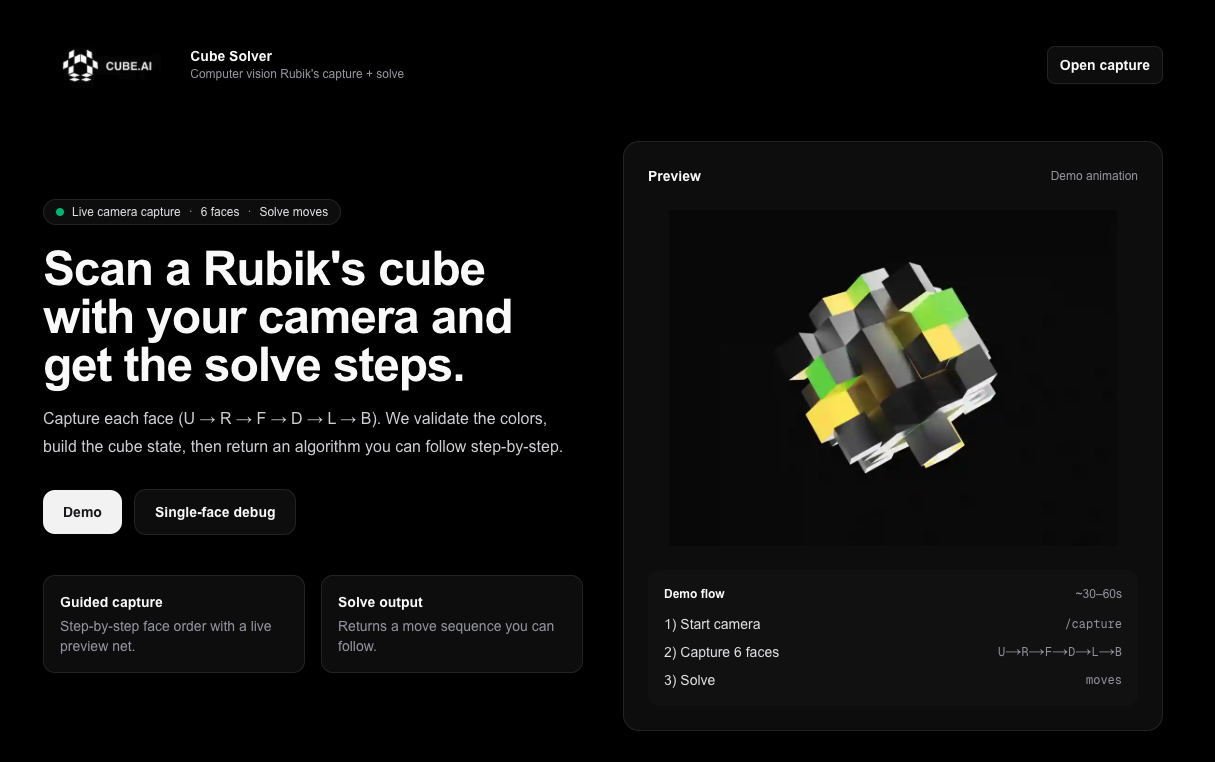
\includegraphics[width=0.95\textwidth,keepaspectratio]{uiimages/home_page.png}}
\caption{Home page.}
\end{figure}

\subsection{6.2 Guided capture (camera and face steps)}\label{frontend-capture}

The capture view walks through faces in a fixed order, shows per-face
hints, exposes camera controls, and surfaces a quality indicator so the
user only accepts frames when the model is confident.

\begin{figure}[htbp]
\centering
\pandocbounded{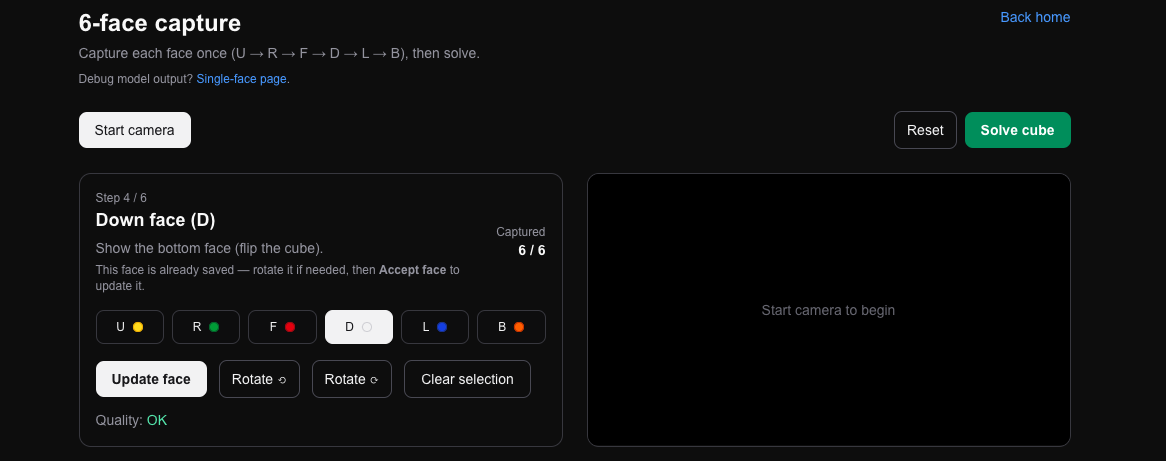
\includegraphics[width=0.95\textwidth,keepaspectratio]{uiimages/1st_section.png}}
\caption{Camera scanning and face capture.}
\end{figure}

\subsection{6.3 Cube preview (two-dimensional net)}\label{frontend-preview}

A net-style preview summarizes the current scan: default center colors
before capture, then filled stickers for the active face (and saved
faces) as predictions arrive. Metadata such as center color, face
confidence, and inference time supports debugging.

\begin{figure}[htbp]
\centering
\pandocbounded{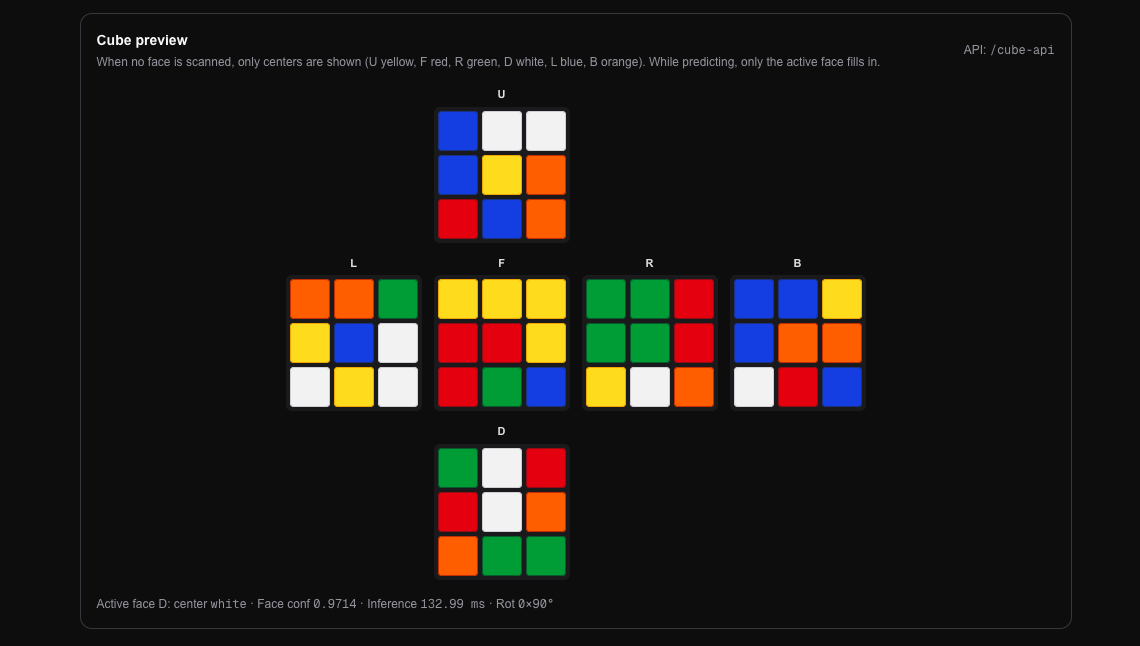
\includegraphics[width=0.95\textwidth,keepaspectratio]{uiimages/second_section.png}}
\caption{Two-dimensional cube preview.}
\end{figure}

\subsection{6.4 Solution moves and animated guidance}\label{frontend-solution}

After all faces are captured, the solver returns an algorithm string and
an optional facelet state. The UI lists the full sequence and offers a
step-by-step panel: each move highlights the next token and plays a
matching animation so the user can follow the solution on a physical
cube.

\begin{figure}[htbp]
\centering
\pandocbounded{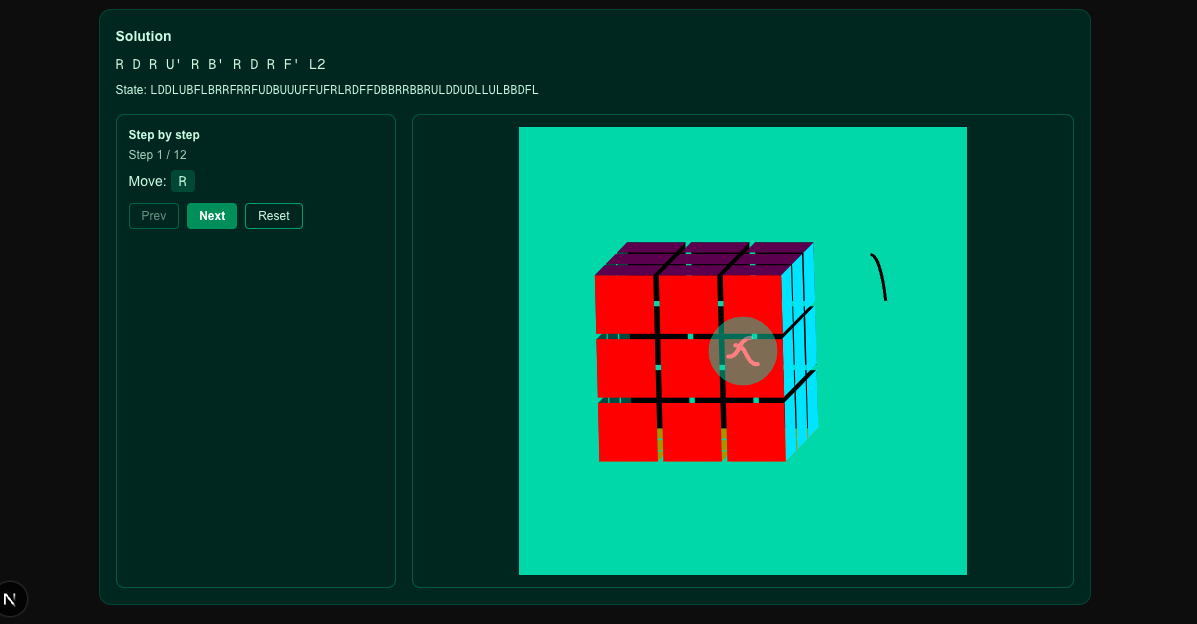
\includegraphics[width=0.95\textwidth,keepaspectratio]{uiimages/third_section.png}}
\caption{Solution algorithm and step-by-step animation.}
\end{figure}

\begin{center}\rule{0.5\linewidth}{0.5pt}\end{center}

\section{7. Lessons Learned}\label{lessons-learned}

\begin{itemize}
\tightlist
\item
  \textbf{Crop precision dominates color accuracy.} Once the classifier
  always saw a centered sticker patch, the color problem became much
  easier --- and many ambiguities collapsed.
\item
  \textbf{Real-world capture is not a ``color sensor''.} Hue alone is
  insufficient because of white balance, exposure, and gamut differences
  between devices. A learned model that has been trained against these
  perturbations is dramatically more robust than fixed thresholds.
\item
  \textbf{Synthetic data plus aggressive photometric augmentation is a
  pragmatic substitute for a large field-collected dataset.} It is
  cheap, balanced, controllable, and --- when the augmentation
  distribution matches the deployment distribution --- generalizes well.
\item
  \textbf{Oriented detection is a natural fit for planar surfaces in
  hand-held captures.} It removes the need for a separate rectification
  step driven by heuristics.
\end{itemize}

\begin{center}\rule{0.5\linewidth}{0.5pt}\end{center}

\section{8. Future Work}\label{future-work}

\begin{itemize}
\tightlist
\item
  \textbf{Adaptive color calibration.} Use the four corner stickers (or
  external markers) for a per-frame illuminant estimate that further
  reduces residual variance.
\item
  \textbf{Real-world dataset expansion.} Continuously collect
  mis-classified real-world stickers, label them, and fold them into the
  training mix to cover edge cases the synthetic distribution misses.
\item
  \textbf{Joint detection + classification model.} Investigate a single
  multi-task network that detects the face and emits the 3x3 color grid
  in one pass, to reduce latency in mobile deployments.
\item
  \textbf{Temporal smoothing.} Aggregate predictions across multiple
  frames while the user holds the cube, to suppress occasional per-frame
  errors.
\end{itemize}

\end{document}
